\section{Three-Dimensional Corridor-Based Collision Avoidance}
\label{sec:corridor}
\subsection{From a Reference Motion to Linear Restrictions}
Assume synchronized reference nodes $\widehat{\bp}_{i,k}$ are available. Their generation is described in Section~\ref{sec:initialization}. The reference determines local boxes that provide conservative linear restrictions for collision avoidance. Each box has three lower and three upper coordinate bounds. Independent six-face expansion produces spatial safe travel corridors (STCs) and relative safe travel corridors (RSTCs) indexed by time.
\begin{figure}[htbp]
\begin{adjustwidth}{-\extralength}{0cm}
\centering\resizebox{\fulllength}{!}{% Native vector artwork; positions are in centimetres.
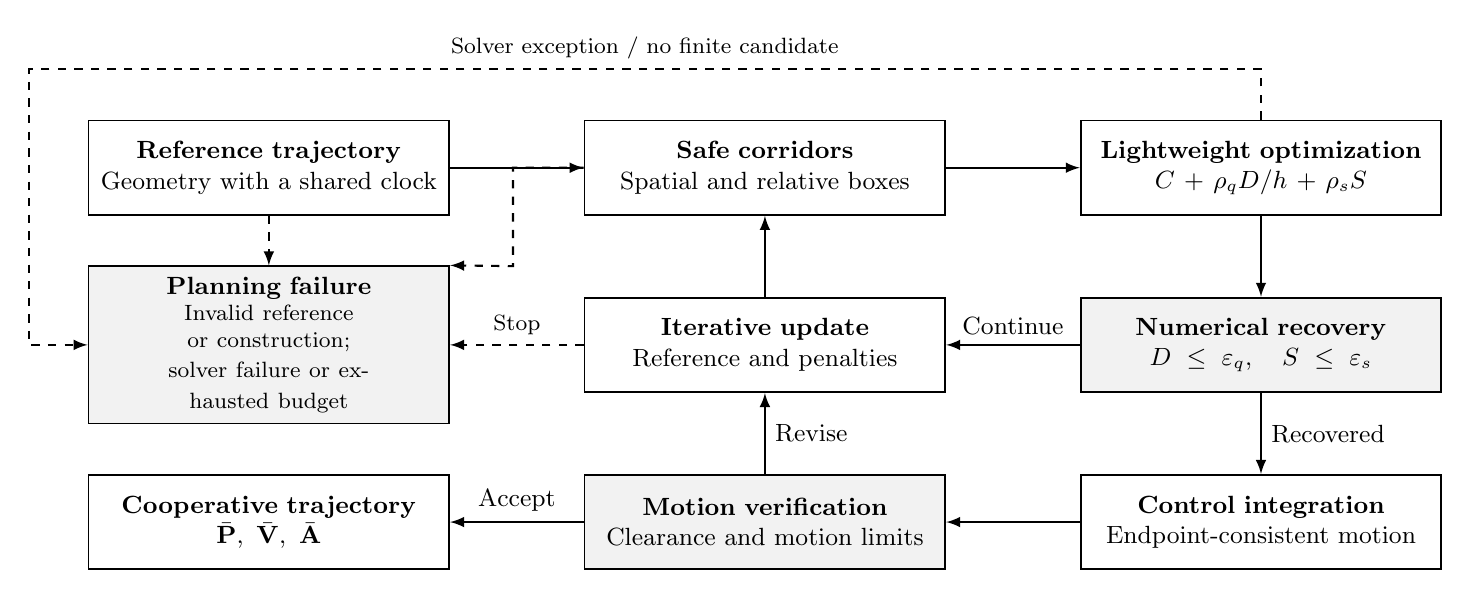
\begin{tikzpicture}[x=1cm,y=1cm,>=latex,font=\small,
 block/.style={draw=black,line width=.65pt,fill=white,text width=4.3cm,minimum height=1.2cm,inner sep=4pt,align=center},
 test/.style={draw=black,line width=.65pt,fill=black!5,text width=4.3cm,minimum height=1.2cm,inner sep=4pt,align=center},
 flow/.style={->,line width=.75pt}]
\node[block] (ref) at (0,0) {\textbf{Reference trajectory}\\Geometry with a shared clock};
\node[block] (corr) at (6.3,0) {\textbf{Safe corridors}\\Spatial and relative boxes};
\node[block] (qp) at (12.6,0) {\textbf{Lightweight optimization}\\$C+\rho_q D/h+\rho_s S$};
\node[block] (update) at (6.3,-2.25) {\textbf{Iterative update}\\Reference and penalties};
\node[test,minimum height=1.35cm] (fail) at (0,-2.25) {\textbf{Planning failure}\\\footnotesize Invalid reference or construction;\\solver failure or exhausted budget};
\node[test] (gate) at (12.6,-2.25) {\textbf{Numerical recovery}\\$D\leq\varepsilon_q,\quad S\leq\varepsilon_s$};
\node[block] (control) at (12.6,-4.5) {\textbf{Control integration}\\Endpoint-consistent motion};
\node[test] (check) at (6.3,-4.5) {\textbf{Motion verification}\\Clearance and motion limits};
\node[block] (out) at (0,-4.5) {\textbf{Cooperative trajectory}\\$\bar{\mathbf P},\ \bar{\mathbf V},\ \bar{\mathbf A}$};
\draw[flow] (ref)--(corr);
\draw[flow] (corr)--(qp);
\draw[flow] (qp)--(gate);
\draw[flow] (gate.west)--node[above]{Continue}(update.east);
\draw[flow] (update.north)--(corr.south);
\draw[flow] (gate.south)--node[right]{Recovered}(control.north);
\draw[flow] (control.west)--(check.east);
\draw[flow] (check.north)--node[right]{Revise}(update.south);
\draw[flow] (check.west)--node[above]{Accept}(out.east);
\draw[flow,dashed] (ref.south)--(fail.north);
\draw[flow,dashed] (update.west)--node[above,font=\footnotesize]{Stop}(fail.east);
\draw[flow,dashed] (corr.west)--(3.1,0)--(3.1,-1.25)--(fail.north east);
\draw[flow,dashed] (qp.north)--(12.6,1.25)
 --node[above,font=\footnotesize]{Solver exception / no finite candidate}(-3.05,1.25)
 --(-3.05,-2.25)--(fail.west);
\end{tikzpicture}
}
\caption{Fixed-horizon cooperative trajectory optimization. The feedback loop revises the reference, penalty weights, and corridor geometry. Numerical recovery triggers control integration, and complete-interval checks determine acceptance. Dashed links mark exits to planning failure.\label{fig:framework}}
\end{adjustwidth}
\end{figure}

\subsection{Spatial Safe Travel Corridors}
To account for movement between nodes, the construction includes temporal padding. For an exactly consistent motion satisfying the Euclidean limits, a reachable-speed bound at node $k$ is
\begin{equation}
 b_{i,k}=\min\{v_{\max},\,\norm{\bv_i^0}_2+a_{\max}t_k,\,
 \norm{\bv_i^f}_2+a_{\max}(T_f-t_k)\}.
 \label{eq:rate}
\end{equation}
Every time in the horizon is at most $h/2$ from a node. With numerical guard $\epsilon_g$, the corresponding padding is
\begin{equation}
 q_{i,k}=\min\left\{\frac{v_{\max}h}{2},\,
 \frac{b_{i,k}h}{2}+\frac{a_{\max}h^2}{8}\right\}+\epsilon_g.
 \label{eq:padding}
\end{equation}
Obstacles are inflated componentwise and the workspace is inset:
\begin{subequations}\label{eq:inflation}\begin{align}
 \mathcal O_b^{i,k}&=[\underline{\mathbf o}_b-(r+c+q_{i,k})\one,
 \overline{\mathbf o}_b+(r+c+q_{i,k})\one],\\
 \mathcal W_{i,k}&=[\underline{\mathbf w}+(r+q_{i,k})\one,
 \overline{\mathbf w}-(r+q_{i,k})\one].
\end{align}\end{subequations}
Axiswise inflation conservatively covers Euclidean obstacle dilation. The STC is a box
\begin{equation}
 \Gamma_{i,k}=[\underline{\boldsymbol\gamma}_{i,k},\overline{\boldsymbol\gamma}_{i,k}]
 \subset\mathcal W_{i,k},\qquad
 \Gamma_{i,k}\cap\mathcal O_b^{i,k}=\varnothing\quad\forall b.
 \label{eq:stc}
\end{equation}

Starting from a valid seed, the algorithm expands the lower and upper faces along $x$, $y$, and $z$ in turn, following incremental local-box growth~\cite{li2022liom}. A step is accepted only if the box remains inside the inset workspace and outside every inflated obstacle. Each face advances by an increment $\Delta_c$, up to a prescribed expansion limit $\ell_s$. When a proposed step intersects an inflated obstacle or leaves the inset workspace, bisection locates the last admissible face position. That face is frozen while the remaining faces continue to grow. Expansion ends when every face is blocked or has reached its limit. Figure~\ref{fig:corridor}(a) illustrates the seed, an intermediate box, and the final corridor.

A reference node can be invalid after temporal inflation even when its uninflated position is free. Such a node is first clipped to the inset workspace. If it remains inside an inflated obstacle, the existing static guide is searched for the nearest admissible projected point. If no guide candidate is available, admissible projections beyond obstacle faces are tested. An admissible seed is required to construct the local corridor.

The resulting static-avoidance constraint is simply
\begin{equation}
 \underline{\boldsymbol\gamma}_{i,k}\leq\bp_{i,k}\leq\overline{\boldsymbol\gamma}_{i,k}.
 \label{eq:withinSTC}
\end{equation}
The spatial box is retained as a hard constraint. Its padding accounts for inter-node motion under the stated speed and acceleration limits.

\subsection{Relative Safe Travel Corridors}
For synchronized UAVs $i$ and $j$, introduce
\begin{equation}
 \mathbf r_{ij,k}=\bp_{i,k}-\bp_{j,k}\in\R^3.
 \label{eq:relative}
\end{equation}
Collision corresponds to this relative vector entering a sphere around the origin. A relative reachable-speed bound and protected radius are
\begin{subequations}\label{eq:relativepadding}\begin{align}
 b_{ij,k}&=\min\{2v_{\max},\,\norm{\bv_i^0-\bv_j^0}_2+2a_{\max}t_k,\nonumber\\[-2pt]
 &\hphantom{=\min\{}\norm{\bv_i^f-\bv_j^f}_2+2a_{\max}(T_f-t_k)\},\\
 R_{ij,k}&=2r+c+\min\left\{v_{\max}h,\,
 \frac{b_{ij,k}h}{2}+\frac{a_{\max}h^2}{4}\right\}+2\epsilon_g.
\end{align}\end{subequations}
\paragraph{Inter-node displacement bound.}
Consider a kinematically consistent motion satisfying the speed and acceleration limits, and let $t_k$ be a nearest node to $t$, with $\tau=|t-t_k|\leq h/2$. Integrating the velocity bound, or integrating from the node using $\norm{\bv_i(t_k)}_2\leq b_{i,k}$ and the acceleration bound, gives
\begin{equation}
 \norm{\bp_i(t)-\bp_{i,k}}_2
 \leq\min\{v_{\max}\tau,\ b_{i,k}\tau+\tfrac12a_{\max}\tau^2\}
 \leq q_{i,k}-\epsilon_g.
 \label{eq:single-displacement}
\end{equation}
The same argument for $\mathbf r_{ij}(t)=\bp_i(t)-\bp_j(t)$ uses relative speed and acceleration bounds $2v_{\max}$ and $2a_{\max}$:
\begin{equation}
 \norm{\mathbf r_{ij}(t)-\mathbf r_{ij,k}}_2
 \leq\min\{2v_{\max}\tau,\ b_{ij,k}\tau+a_{\max}\tau^2\}.
 \label{eq:relative-displacement}
\end{equation}
Substitution of $\tau\leq h/2$ yields the $h^2/8$ and $h^2/4$ terms in~\eqref{eq:padding} and~\eqref{eq:relativepadding}. By the triangle inequality, nodal clearance enlarged by the corresponding padding is sufficient to preserve the required continuous-time clearance over the neighboring half intervals. This conclusion applies to kinematically consistent motion satisfying the stated limits. Relaxed candidates pass through the reconstruction and acceptance stages in Section~\ref{sec:liom}.

Relative boxes are unnecessary when the corresponding STCs already separate all possible positions. Define
\begin{equation}
 \mathbf g_{ij,k}=\max\{\underline{\boldsymbol\gamma}_{i,k}-\overline{\boldsymbol\gamma}_{j,k},\,
 \underline{\boldsymbol\gamma}_{j,k}-\overline{\boldsymbol\gamma}_{i,k},\,\mathbf0\}.
 \label{eq:screen}
\end{equation}
Only pair--node triples with $\norm{\mathbf g_{ij,k}}_2<R_{ij,k}$ belong to the active set $\mathcal A$. The screening test covers every relative position admitted by the two spatial boxes.

For each active triple, a box $\mathcal R_{ij,k}=[\underline{\boldsymbol\eta}_{ij,k},\overline{\boldsymbol\eta}_{ij,k}]$ is grown around the reference relative position, subject to
\begin{equation}
 \norm{\max\{\underline{\boldsymbol\eta}_{ij,k},-\overline{\boldsymbol\eta}_{ij,k},\mathbf0\}}_2
 \geq R_{ij,k}.
 \label{eq:relativebox}
\end{equation}
The left side is the exact minimum Euclidean distance from the origin to the box. Thus every point in the unrelaxed relative box lies outside the protected sphere. The relative box grows through the same six-face procedure, with step $\Delta_c$ and expansion limit $\ell_r$. Each proposed face movement is accepted only while~\eqref{eq:relativebox} holds. A seed inside the protected sphere is first displaced radially beyond its boundary by a small guard distance. For coincident seeds, the direction is obtained from the assigned start--goal geometry. Figure~\ref{fig:corridor}(b) shows the construction in relative-position space.
\begin{figure}[htbp]
\begin{adjustwidth}{-\extralength}{0cm}
\centering\resizebox{\fulllength}{!}{% Oblique, orthographic vector construction. Solid/dashed lines encode state.
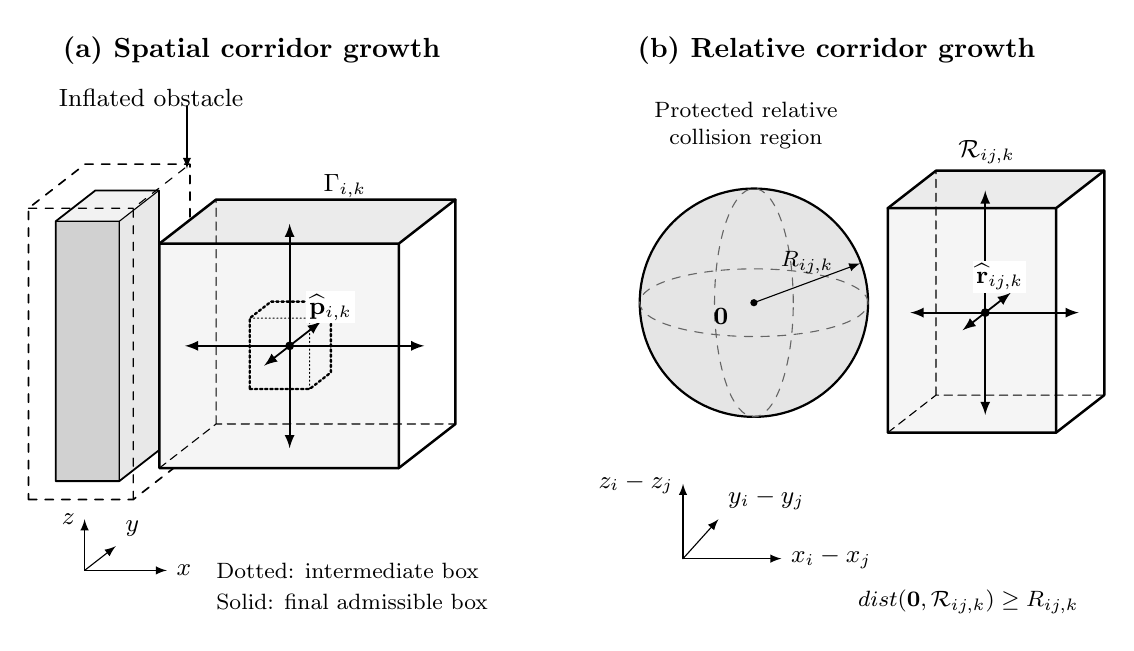
\begin{tikzpicture}[x=1cm,y=1cm,>=latex,font=\small,line cap=round,line join=round]
% Panel A: true 3-D cuboids in an explicit oblique basis.
\node[anchor=west,font=\bfseries] at (-.4,5.55) {(a) Spatial corridor growth};
\begin{scope}[x={(.95cm,0cm)},y={(.36cm,.28cm)},z={(0cm,1cm)}]
% Inflated obstacle: solid core and dashed clearance boundary.
\fill[black!18] (-.5,.3,0)--(.35,.3,0)--(.35,.3,3.3)--(-.5,.3,3.3)--cycle;
\fill[black!9] (.35,.3,0)--(.35,1.7,0)--(.35,1.7,3.3)--(.35,.3,3.3)--cycle;
\fill[black!5] (-.5,.3,3.3)--(.35,.3,3.3)--(.35,1.7,3.3)--(-.5,1.7,3.3)--cycle;
\draw[line width=.65pt] (-.5,.3,0)--(.35,.3,0)--(.35,1.7,0)--(.35,1.7,3.3)--(-.5,1.7,3.3)--(-.5,.3,3.3)--cycle;
\draw (.35,.3,0)--(.35,.3,3.3)--(.35,1.7,3.3) (-.5,.3,3.3)--(.35,.3,3.3);
\draw[dashed,line width=.6pt] (-.75,0,-.15)--(.65,0,-.15)--(.65,2,-.15)--(.65,2,3.55)--(-.75,2,3.55)--(-.75,0,3.55)--cycle;
\draw[dashed] (.65,0,-.15)--(.65,0,3.55)--(.65,2,3.55) (-.75,0,3.55)--(.65,0,3.55);
% Final corridor.
\fill[black!4] (1,0,.25)--(4.2,0,.25)--(4.2,0,3.1)--(1,0,3.1)--cycle;
\fill[black!8] (1,0,3.1)--(4.2,0,3.1)--(4.2,2,3.1)--(1,2,3.1)--cycle;
\draw[line width=.9pt] (1,0,.25)--(4.2,0,.25)--(4.2,2,.25)--(4.2,2,3.1)--(1,2,3.1)--(1,0,3.1)--cycle;
\draw[line width=.9pt] (4.2,0,.25)--(4.2,0,3.1)--(4.2,2,3.1) (1,0,3.1)--(4.2,0,3.1);
\draw[densely dashed] (1,0,.25)--(1,2,.25)--(4.2,2,.25) (1,2,.25)--(1,2,3.1);
% Seed and early growth stage.
\draw[densely dotted,line width=.85pt] (2,.55,1.1)--(2.8,.55,1.1)--(2.8,1.3,1.1)--(2.8,1.3,2)--(2,1.3,2)--(2,.55,2)--cycle;
\draw[densely dotted] (2.8,.55,1.1)--(2.8,.55,2)--(2.8,1.3,2) (2,.55,2)--(2.8,.55,2);
\fill (2.4,.9,1.55) circle (1.6pt);
\foreach \a/\b/\c in {1/.9/1.55,4.2/.9/1.55,2.4/0/1.55,2.4/2/1.55,2.4/.9/.25,2.4/.9/3.1}
 {\draw[->,line width=.65pt] (2.4,.9,1.55)--(\a,\b,\c);}
\node[anchor=west,fill=white,inner sep=1pt] at (2.9,.15,2.25) {$\widehat{\mathbf p}_{i,k}$};
\node at (3.1,1,3.55) {$\Gamma_{i,k}$};
% Small coordinate triad.
\draw[->] (0,0,-1.05)--(1.1,0,-1.05) node[right] {$x$};
\draw[->] (0,0,-1.05)--(0,1.1,-1.05) node[above right] {$y$};
\draw[->] (0,0,-1.05)--(0,0,-.4) node[left] {$z$};
\end{scope}
\node[anchor=west] at (-.45,4.95) {Inflated obstacle};
\draw[->,thin] (1.3,4.85)--(1.3,4.05);
\node[anchor=west,font=\footnotesize] at (1.55,-1.05) {Dotted: intermediate box};
\node[anchor=west,font=\footnotesize] at (1.55,-1.45) {Solid: final admissible box};
% Panel B relative space; a 3-D sphere is shown with meridians.
\begin{scope}[shift={(8.3,0)}]
\node[anchor=west,font=\bfseries] at (-1.4,5.55) {(b) Relative corridor growth};
\coordinate (O) at (.2,2.35);
\fill[black!10] (O) circle (1.45);
\draw[line width=.8pt] (O) circle (1.45);
\draw[black!60,dashed] (O) ellipse (1.45 and .43);
\draw[black!60,dashed] (O) ellipse (.5 and 1.45);
\fill (O) circle (1.3pt);
\draw[->] (O)--node[above,font=\footnotesize] {$R_{ij,k}$} (1.55,2.85);
\node[anchor=east] at (0,2.18) {$\mathbf0$};
\node[align=center,font=\footnotesize] at (.1,4.6) {Protected relative\\collision region};
\begin{scope}[x={(.95cm,0cm)},y={(.36cm,.28cm)},z={(0cm,1cm)}]
\fill[black!4] (2,0,.7)--(4.25,0,.7)--(4.25,0,3.55)--(2,0,3.55)--cycle;
\fill[black!8] (2,0,3.55)--(4.25,0,3.55)--(4.25,1.7,3.55)--(2,1.7,3.55)--cycle;
\draw[line width=.9pt] (2,0,.7)--(4.25,0,.7)--(4.25,1.7,.7)--(4.25,1.7,3.55)--(2,1.7,3.55)--(2,0,3.55)--cycle;
\draw[line width=.9pt] (4.25,0,.7)--(4.25,0,3.55)--(4.25,1.7,3.55) (2,0,3.55)--(4.25,0,3.55);
\draw[densely dashed] (2,0,.7)--(2,1.7,.7)--(4.25,1.7,.7) (2,1.7,.7)--(2,1.7,3.55);
\fill (3,.8,2) circle (1.6pt);
\foreach \a/\b/\c in {2/.8/2,4.25/.8/2,3/0/2,3/1.7/2,3/.8/.7,3/.8/3.55}
 {\draw[->,line width=.65pt] (3,.8,2)--(\a,\b,\c);}
\node[anchor=west,fill=white,inner sep=1pt] at (3.1,.1,2.65) {$\widehat{\mathbf r}_{ij,k}$};
\node at (3,.85,4.02) {$\mathcal R_{ij,k}$};
\end{scope}
\draw[->] (-.7,-.9)--(.55,-.9) node[right] {$x_i-x_j$};
\draw[->] (-.7,-.9)--(-.25,-.4) node[above right] {$y_i-y_j$};
\draw[->] (-.7,-.9)--(-.7,.05) node[left] {$z_i-z_j$};
\node[anchor=west,font=\footnotesize] at (1.4,-1.45) {$\operatorname{dist}(\mathbf0,\mathcal R_{ij,k})\geq R_{ij,k}$};
\end{scope}
\end{tikzpicture}
}
\caption{Six-face corridor growth. (a) A spatial box expands from a reference seed; each face stops at an inflated obstacle, the inset workspace, or its expansion limit. (b) A relative box expands while remaining outside the protected sphere. The arrows denote independent growth along the positive and negative coordinate directions.\label{fig:corridor}}
\end{adjustwidth}
\end{figure}

\subsection{Slackened Relative Bounds}
Independent spatial and relative boxes can conflict. One nonnegative scalar $\delta_{ij,k}$ therefore relaxes all three relative coordinates of each active triple:
\begin{equation}
 \underline{\boldsymbol\eta}_{ij,k}-\delta_{ij,k}\one
 \leq\bp_{i,k}-\bp_{j,k}
 \leq\overline{\boldsymbol\eta}_{ij,k}+\delta_{ij,k}\one,
 \qquad\delta_{ij,k}\geq0.
 \label{eq:relativeSlack}
\end{equation}
The scalar slack, measured in length units, quantifies compatibility with the selected relative box. A positive value can occur even when the UAVs remain physically separated, since the box is conservative. At zero slack, active pairs satisfy the protected nodal-distance condition through~\eqref{eq:relativebox}, and screened pairs are separated by their spatial boxes. The final integrated motion is checked against the original physical clearance conditions.
